% =====================================================================
%  GCN Toy Project - Project Report (about 5-6 pages)
%  Compile from report/:  pdflatex report.tex   (figures: ../figures/)
% =====================================================================
\documentclass[11pt,a4paper]{article}

\usepackage[T1]{fontenc}
\usepackage[utf8]{inputenc}
\usepackage{lmodern}
\usepackage{microtype}
\usepackage[a4paper,margin=2.3cm]{geometry}
\usepackage{amsmath,amssymb,bm}
\usepackage{booktabs}
\usepackage{graphicx}
\graphicspath{{../figures/}{figures/}}  % works from report/ or the repo root
\usepackage{float}
\usepackage{caption}
\usepackage{subcaption}
\captionsetup{font=small,labelfont=bf}
\usepackage{enumitem}
\setlist{itemsep=1pt,topsep=3pt}
\usepackage{tikz}
\usetikzlibrary{positioning,arrows.meta}
\usepackage{xcolor}
\usepackage[colorlinks=true,linkcolor=blue!50!black,urlcolor=blue!50!black]{hyperref}

\setlength{\parskip}{4pt}
\setlength{\parindent}{0pt}

\newcommand{\Ahat}{\hat{A}}
\newcommand{\Dhat}{\hat{D}}
\newcommand{\Anorm}{\tilde{A}}
\newcommand{\R}{\mathbb{R}}

\begin{document}

% ---------------------------------------------------------------------
\begin{center}
  {\LARGE\bfseries Node Classification with a\\[2pt] Three-Layer Graph Convolutional Network}\\[8pt]
  % TODO: replace with the team members' names (and register numbers)
  {\large Member 1, Member 2, Member 3 \quad\textbar\quad Machine Learning with Graphs}\\[2pt]
  {\small Code: \url{https://github.com/Gowreesh1905/GCN_ML_with_graphs}}
\end{center}
\vspace{4pt}

% =====================================================================
\section{What This Project Does}

Many datasets are naturally \emph{graphs}: people connected by friendships, papers connected by citations, students connected by study groups. In such data, a node's connections often say something about the node itself. An ordinary neural network looks at each example on its own and ignores these connections. A \textbf{Graph Convolutional Network (GCN)} is designed to use them: each node updates its representation by combining its own features with those of its neighbours.

In this project we built a three-layer GCN \textbf{from scratch in PyTorch}, using only matrix operations (no graph library such as PyTorch Geometric), so that every mathematical step is visible in the code. The model solves a \textbf{node classification} task: given a graph of 200 students in which only some students' results are known, predict whether each remaining student will \emph{Pass} or \emph{Fail}.

The project then asks four questions:
\begin{enumerate}
  \item Does the GCN do better than a plain neural network that ignores the graph?
  \item Does it do better than simply copying the labels of a student's neighbours, which needs no learning at all?
  \item How does the number of GCN layers (1, 2 or 3) affect accuracy?
  \item How much does the answer depend on how reliable the graph is?
\end{enumerate}

% =====================================================================
\section{The Dataset}

The data is \textbf{synthetic}, generated by the code with a fixed random seed so that every run is identical.

\textbf{Nodes (students).} There are 200 students: 110 who pass and 90 who fail. Each student has three features: \emph{study hours}, \emph{attendance} and \emph{assignment score}. Passing students score higher on average, but the two groups \textbf{overlap strongly}: many failing students study as much as passing ones. This is deliberate. If the features separated the groups perfectly, any model would be perfect and the graph would have nothing to add.

\textbf{Edges (study groups).} Two students are connected with probability 0.06 if they have the same result and 0.015 if they do not. This produces 753 edges, about 7.5 friends per student, and $608/753 = 81\%$ of edges join students with the same result. This tendency of connected nodes to share a label is called \textbf{homophily}, and it is exactly what a GCN can take advantage of. (One student happens to have no connections.)

\textbf{Why these probabilities?} They were chosen for two properties, before any model was trained: a sparse graph with a realistic number of friends per student (about 7.5), and a homophily of about 0.8, similar to the well-known Cora citation benchmark (0.81). Because 0.8 is only one possible value, Section~\ref{sec:sweep} repeats the main experiment on graphs with homophily from 0.9 down to 0.5.

\textbf{Labelled and unlabelled students.} The students are split into 120 \emph{training} nodes (labels visible to the model), 40 \emph{validation} nodes (used to decide when to stop training) and 40 \emph{test} nodes (labels hidden and used only to measure accuracy). The model always sees the whole graph, including the connections of test students; only their labels are hidden. This is called a \emph{transductive} setting. Features are standardized using the mean and standard deviation of the training nodes only, so no information leaks from the test set.

\begin{figure}[H]
\centering
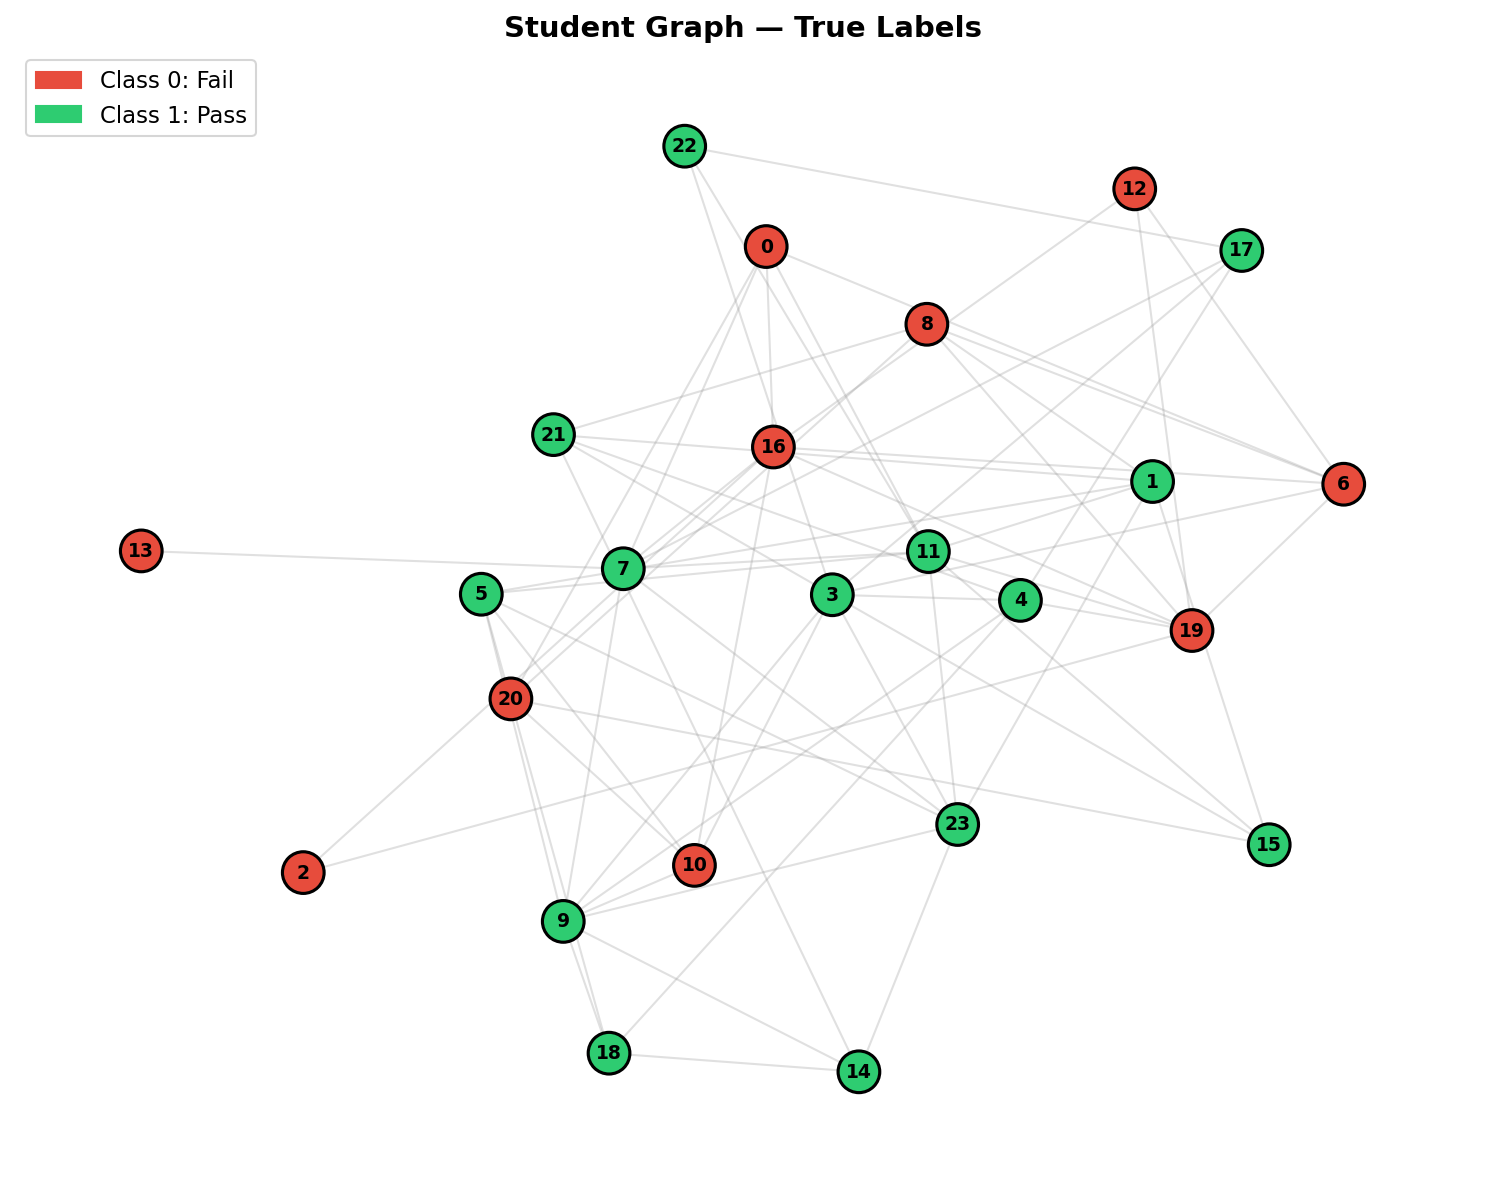
\includegraphics[width=0.52\textwidth]{fig1_graph_true_labels.png}
\caption{The student graph. Green = Pass, red = Fail. Students mostly connect to others with the same result, so the two groups form two loose clusters.}
\label{fig:graph}
\end{figure}

% =====================================================================
\section{How a GCN Works}

The graph is stored as an \textbf{adjacency matrix} $A \in \R^{200 \times 200}$, where $A_{ij}=1$ if students $i$ and $j$ are connected and $0$ otherwise. Because study groups go both ways, $A$ is symmetric. The features are stored in a matrix $X \in \R^{200 \times 3}$, one row per student. Before training, the adjacency matrix is prepared in three steps.

\textbf{Step 1: add self-loops.} We compute $\Ahat = A + I$. Without this, a node that averages over its neighbours would ignore its \emph{own} features. Adding the identity matrix makes every node its own neighbour. (It also gives the one unconnected student something to average: itself.)

\textbf{Step 2: count degrees.} The degree matrix $\Dhat$ is diagonal, with $\Dhat_{ii}$ equal to the number of neighbours of node $i$ (including itself).

\textbf{Step 3: normalize.}
\begin{equation}
  \Anorm = \Dhat^{-1/2}\,\Ahat\,\Dhat^{-1/2},
  \qquad\text{so}\qquad
  \Anorm_{ij} = \frac{1}{\sqrt{\hat d_i \, \hat d_j}} \ \text{ if $i$ and $j$ are connected.}
\end{equation}
Without normalization, a student with many friends would add up many feature vectors and end up with much larger values than a student with few friends. Dividing by the degrees turns the sum into a balanced, weighted average, which keeps values on a similar scale for every node and across layers.

\textbf{The GCN layer.} With $\Anorm$ prepared, one GCN layer is a single line of maths:
\begin{equation}
  H^{(l+1)} = \sigma\big(\,\Anorm\, H^{(l)}\, W^{(l)}\,\big).
\end{equation}
Reading it from left to right:
\begin{itemize}
  \item $\Anorm H^{(l)}$ is \textbf{aggregation}: each node's new vector is a weighted average of its own and its neighbours' current vectors ($H^{(0)} = X$).
  \item Multiplying by $W^{(l)}$ is a \textbf{learned linear transformation}, the part that training adjusts.
  \item $\sigma$ is the ReLU activation, which adds non-linearity. It is \emph{not} applied after the last layer, because the output must be raw class scores (\emph{logits}), which can be negative.
\end{itemize}

\textbf{A tiny example.} Take four students connected in a ring, 0--1--2--3--0. After adding self-loops every node has 3 neighbours (two others and itself), so every non-zero entry of $\Anorm$ is $1/\sqrt{3 \cdot 3} = 1/3$. Student 0 is connected to students 1 and 3, so its new \emph{study hours} value is the average $(5 + 8 + 6)/3 = 6.33$ of itself and its neighbours. One multiplication by $\Anorm$ has blended each student with their study group. Stacking layers repeats this, so after $k$ layers a node is influenced by everyone up to $k$ steps away (its \emph{receptive field}).

\textbf{Why this helps here.} A single student's features are ambiguous because the groups overlap. But their study group is mostly made up of students with the same result, so the \emph{average} over the group is a much more reliable signal than the student alone. This is the effect the experiments measure.

% =====================================================================
\section{The Model and How It Is Trained}

The main model has three GCN layers. The first maps the 3 input features to 8 hidden values, the second maps 8 to 8, and the third maps 8 values to 2 scores, one per class (Figure~\ref{fig:arch}). The layers have $3{\times}8 + 8{\times}8 + 8{\times}2 = 104$ weights in total.

\begin{figure}[H]
\centering
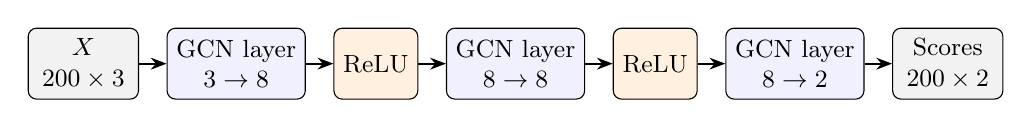
\begin{tikzpicture}[
  box/.style={draw, rounded corners=3pt, minimum height=0.9cm, minimum width=1.75cm, align=center, font=\small, fill=blue!6},
  act/.style={draw, rounded corners=3pt, minimum height=0.9cm, minimum width=1.0cm, align=center, font=\small, fill=orange!12},
  io/.style={draw, rounded corners=3pt, minimum height=0.9cm, minimum width=1.4cm, align=center, font=\small, fill=black!5},
  arr/.style={-{Stealth[length=2mm]}, thick},
  node distance=0.35cm
]
  \node[io]  (x)  {$X$\\$200 \times 3$};
  \node[box, right=of x]  (g1) {GCN layer\\$3 \to 8$};
  \node[act, right=of g1] (r1) {ReLU};
  \node[box, right=of r1] (g2) {GCN layer\\$8 \to 8$};
  \node[act, right=of g2] (r2) {ReLU};
  \node[box, right=of r2] (g3) {GCN layer\\$8 \to 2$};
  \node[io, right=of g3] (z) {Scores\\$200 \times 2$};
  \draw[arr] (x) -- (g1);  \draw[arr] (g1) -- (r1); \draw[arr] (r1) -- (g2);
  \draw[arr] (g2) -- (r2); \draw[arr] (r2) -- (g3); \draw[arr] (g3) -- (z);
\end{tikzpicture}
\caption{The three-layer GCN. Every layer uses the same normalized adjacency $\Anorm$.}
\label{fig:arch}
\end{figure}

\textbf{Training.} The model processes the whole graph at once and produces two scores for every student. Softmax turns the scores into probabilities, and the prediction is the class with the higher probability. The \textbf{cross-entropy loss} is computed only on the 120 training students, and the Adam optimizer (learning rate 0.01) updates the weights to reduce it. Two standard safeguards against overfitting are used:
\begin{itemize}
  \item \textbf{Dropout and weight decay.} During training, half of the hidden values are randomly set to zero at each step (dropout 0.5), and large weights are lightly penalized (weight decay $5\times10^{-4}$). Both stop the model from relying too heavily on any single pattern.
  \item \textbf{Early stopping.} After every epoch the loss on the 40 validation students is checked. Training stops once it has not improved for 30 epochs, and the model is reset to the weights from its best epoch. This also removes the need to guess how many epochs to train for.
\end{itemize}

\textbf{Models compared.} All of them are trained in exactly the same way.
\begin{itemize}
  \item \textbf{MLP}: an ordinary two-layer neural network that sees only each student's own features and \emph{ignores the graph}. It shows how far the features alone can go.
  \item \textbf{GCN-1, GCN-2, GCN-3}: GCNs with 1, 2 and 3 layers, to study the effect of depth.
  \item \textbf{GCN-3 without regularization}: the same model with no dropout, no weight decay and no early stopping (a fixed 200 epochs), to check whether the safeguards matter.
  \item \textbf{GCN-3 on a random graph}: the real study groups replaced by random connections (same number of edges). This tests whether the GCN relies on the graph being meaningful.
  \item \textbf{Neighbour vote}: a baseline with no features and no learning. Each test student is given the label held by most of their \emph{labelled} neighbours (ties and students with no labelled neighbours get the most common training label). It measures how much the graph alone can do.
\end{itemize}

\textbf{Fair evaluation.} Every experiment is repeated with \textbf{10 random seeds}. Each seed draws a \emph{new} train/validation/test split and new starting weights, and the results are reported as the mean and standard deviation over the 10 runs. With 40 test students per run, one mistake changes accuracy by 2.5 percentage points.

% =====================================================================
\section{Results}

\begin{table}[H]
\centering
\caption{Accuracy over 10 seeds (mean $\pm$ standard deviation, 40 test students per seed).}
\label{tab:results}
\begin{tabular}{@{}lcccc@{}}
\toprule
Model & Uses & Weights & Train accuracy & Test accuracy \\
\midrule
MLP                        & Features         & 50  & $78.8\% \pm 2.7$ & $77.8\% \pm 5.2$ \\
Neighbour vote             & Graph + labels   & 0   & ---              & $87.0\% \pm 6.2$ \\
GCN-1                      & Features + graph & 6   & $90.9\% \pm 2.2$ & $90.5\% \pm 5.0$ \\
GCN-2                      & Features + graph & 40  & $95.5\% \pm 1.9$ & $92.5\% \pm 4.3$ \\
GCN-3                      & Features + graph & 104 & $95.7\% \pm 1.9$ & $\mathbf{94.0\% \pm 4.4}$ \\
GCN-3, no regularization   & Features + graph & 104 & $96.3\% \pm 1.7$ & $94.3\% \pm 4.3$ \\
GCN-3, random graph        & Features + random graph & 104 & ---       & $50.8\% \pm 10.7$ \\
\bottomrule
\end{tabular}
\end{table}

\begin{figure}[H]
\centering
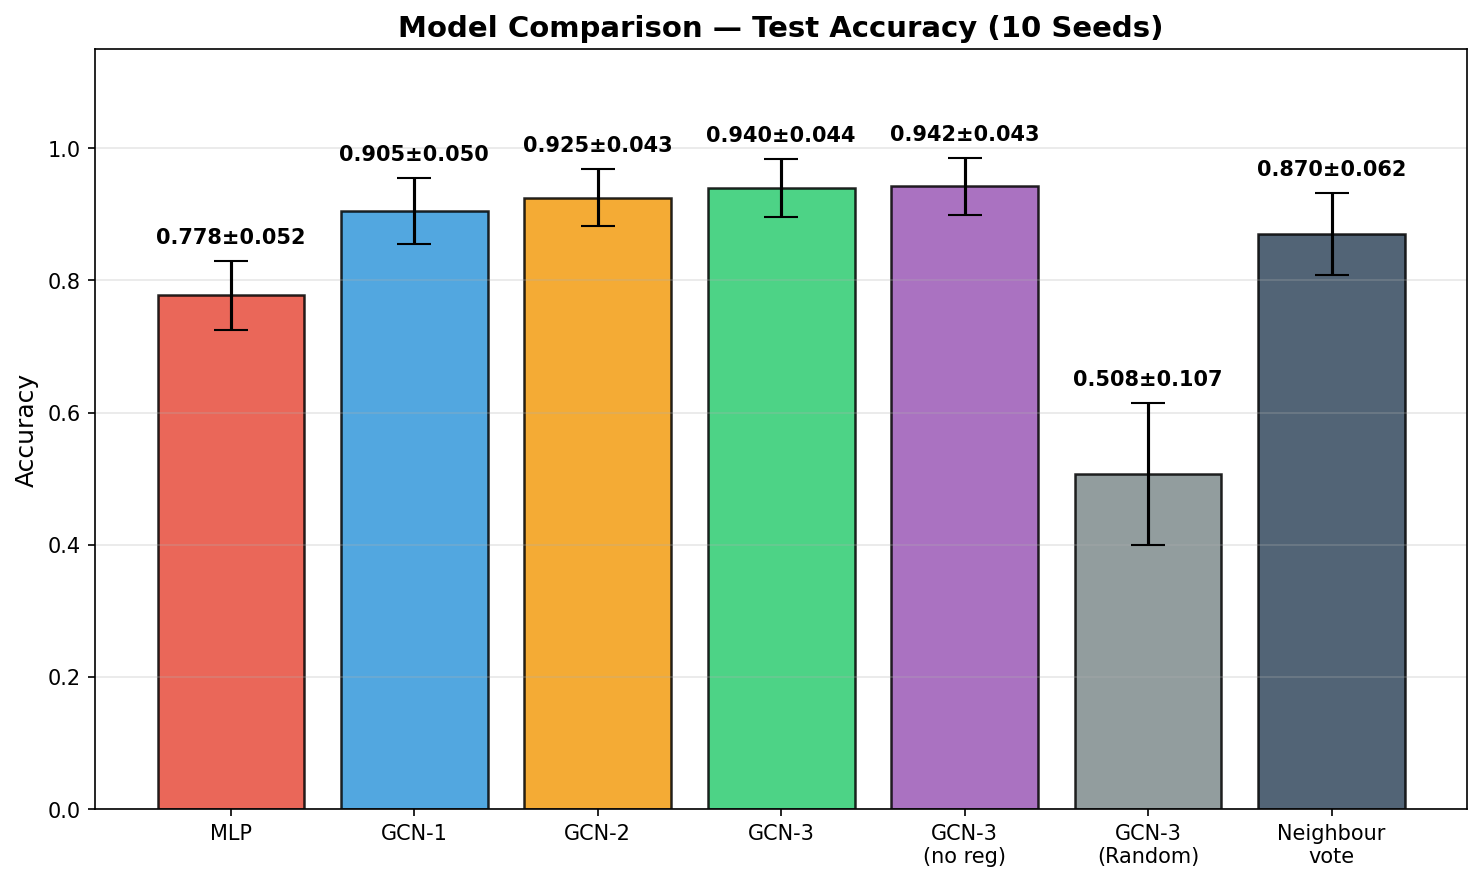
\includegraphics[width=0.68\textwidth]{fig8_model_comparison_accuracy.png}
\caption{Test accuracy of every model on the main graph (homophily 0.81, 10 seeds).}
\label{fig:results}
\end{figure}

\subsection{How Reliable Must the Graph Be?}
\label{sec:sweep}

To see how much the results depend on the chosen edge probabilities, the experiment was repeated on five graphs with homophily 0.9, 0.8, 0.7, 0.6 and 0.5. Everything else stays the same: the same students and features, the same splits, and the same expected number of edges (about 750). Only the share of edges joining students with the same result changes. At 0.5 the graph carries no information about the labels at all.

\begin{table}[H]
\centering
\caption{Test accuracy as homophily falls (10 seeds per level). The MLP ignores the graph, so its accuracy does not change.}
\label{tab:sweep}
\begin{tabular}{@{}lccccc@{}}
\toprule
Homophily & 0.90 & 0.80 & 0.70 & 0.60 & 0.50 \\
\midrule
MLP (features only)          & 77.8\% & 77.8\% & 77.8\% & \textbf{77.8\%} & \textbf{77.8\%} \\
Neighbour vote (graph only)  & 94.5\% & 86.8\% & 78.8\% & 66.5\% & 51.3\% \\
GCN-1                        & 95.2\% & 89.5\% & 82.3\% & 72.7\% & 60.0\% \\
GCN-3                        & \textbf{99.5\%} & \textbf{93.2\%} & \textbf{84.3\%} & 68.8\% & 52.5\% \\
\bottomrule
\end{tabular}
\end{table}

\begin{figure}[H]
\centering
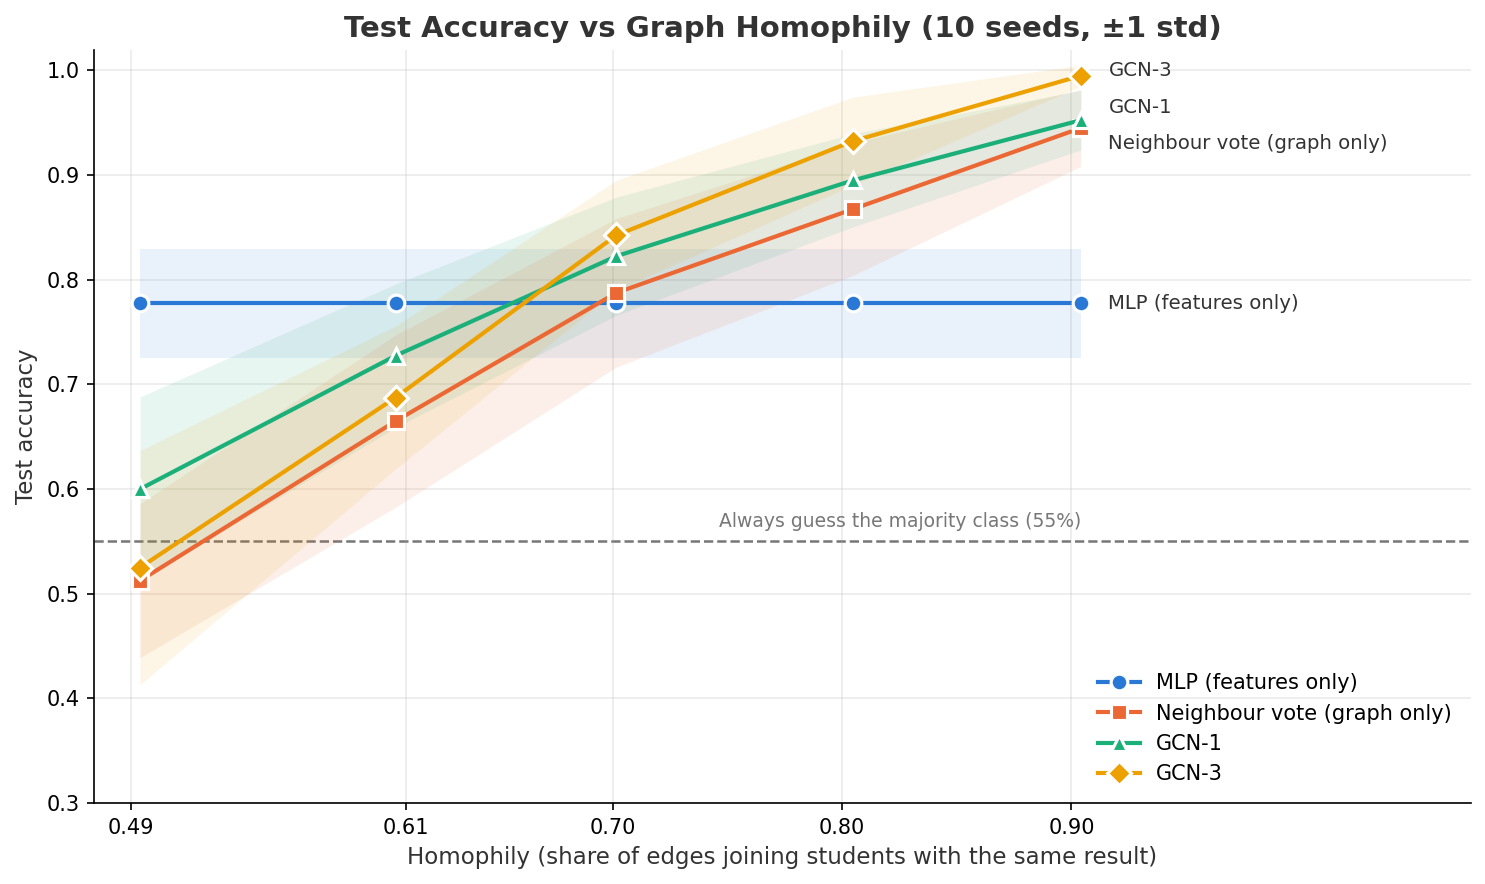
\includegraphics[width=0.74\textwidth]{fig11_homophily_sweep.png}
\caption{Test accuracy against homophily. Shaded bands show $\pm 1$ standard deviation over the 10 seeds. The GCN lines cross the MLP line between homophily 0.6 and 0.7.}
\label{fig:sweep}
\end{figure}

% =====================================================================
\section{What the Results Mean}

\textbf{1. Features alone are not enough.} The MLP, which sees each student in isolation, reaches only 77.8\%. With overlapping features, many students are genuinely ambiguous on their own.

\textbf{2. The graph alone already does a lot.} The neighbour vote uses no features and learns nothing, yet reaches 87.0\%, ahead of the MLP. With 81\% of edges joining students with the same result, simply copying what most of a student's labelled friends got is usually right. This is an important check: much of the GCN's advantage over the MLP comes from the graph itself, not from anything clever the GCN does.

\textbf{3. The GCN does best by combining both.} GCN-3 reaches 94.0\%, seven points above the vote and sixteen above the MLP, and it beats the MLP on all 10 splits. It has two advantages over the vote. First, it also uses each student's own features, which helps when their neighbours are split (13 students have exactly half of their neighbours in each class) or when they have no labelled neighbours. Second, it averages \emph{features} rather than labels, so it learns something even from neighbours whose labels are hidden; the vote ignores those.

\textbf{4. A GCN is only as good as its graph.} Table~\ref{tab:sweep} and Figure~\ref{fig:sweep} show that the GCN beats the neighbour vote at every homophily level, but it beats the plain MLP only while homophily is about 0.7 or higher. Below that, the GCN is \emph{worse than ignoring the graph}: at homophily 0.5, GCN-3 scores 52.5\% against the MLP's 77.8\%. The reason is in the layer rule $\Anorm H W$: every layer averages a student with their neighbours, and the model has no way to switch this off. When neighbours are unreliable, the averaging drowns out the student's own useful features. The random-graph experiment (50.8\%) shows the same effect.

\textbf{5. Depth amplifies the graph, for better or worse.} On reliable graphs, extra layers help: GCN-3 beats GCN-1 at homophily 0.7 and above, reaching 99.5\% at 0.9, because it gathers evidence from friends of friends. On unreliable graphs, the extra layers hurt: GCN-3 falls below GCN-1 at 0.6 and 0.5, because three rounds of averaging mix in more students of the wrong class than one round does. On the main graph the differences between depths (90.5\%, 92.5\%, 94.0\%) are smaller than the variation between splits, so they are a trend rather than a firm result. There is no sign of over-smoothing, where repeated averaging makes all students look alike.

\textbf{6. Regularization makes no measurable difference here.} GCN-3 with and without dropout, weight decay and early stopping scores 94.0\% and 94.3\%, with training accuracy only slightly above test accuracy, so the model is not overfitting: 120 labelled students are enough for 104 weights. Early stopping is still useful because it chooses the training length automatically. On seed 42, GCN-3 stopped after 142 epochs and kept its weights from epoch 112, while the 1-layer GCN typically keeps improving for about 440 epochs. The few students GCN-3 still gets wrong sit where the Pass and Fail clusters meet, where a student's study group is itself mixed.

% =====================================================================
\section{Limitations}

\begin{itemize}
  \item \textbf{Synthetic data.} The homophily and the amount of feature overlap are parameters we chose. The homophily sweep shows how strongly the conclusions depend on the first; on real data the GCN's advantage could be smaller or larger.
  \item \textbf{A simple graph baseline.} The neighbour vote is the simplest way to use the graph. Stronger label-based methods, such as label propagation, which passes labels along several hops, might close part of the gap to the GCN.
  \item \textbf{Small differences between depths.} With 40 test students per split, the gaps between GCN-1, GCN-2 and GCN-3 on the main graph are within the noise of the experiment.
  \item \textbf{Fixed graph and features.} For each homophily level, all seeds share one graph and one set of features; only the split and the starting weights vary.
  \item \textbf{Dense matrices.} The $200 \times 200$ adjacency matrix is stored in full. This is clear for learning but would not scale to graphs with millions of nodes, which need sparse matrices.
\end{itemize}

\textbf{Possible next steps:} compare against label propagation; try GCN variants that keep a separate weight for a node's own features (such as GraphSAGE), which can learn to rely on the features when the graph is unreliable; and test the same code on a real benchmark graph such as Cora.

% =====================================================================
\section{Conclusion}

This project implemented a Graph Convolutional Network from first principles and showed what each step does: self-loops keep a node's own features, normalization keeps values balanced across nodes, and the layer rule $\Anorm H W$ is simply \emph{average over neighbours, then transform}. On a graph where 81\% of connections join students with the same result, features alone gave 78\% accuracy and the graph alone (a neighbour vote) gave 87\%; the GCN, which combines both, reached 94\%. The homophily sweep showed the limit of this: the GCN helps only when the graph is reliable enough, roughly when at least 70\% of connections join similar nodes. Below that, a plain GCN does worse than ignoring the graph, and deeper GCNs do worse still. A GCN is a powerful way to combine features with structure, but only when the structure is trustworthy.

% ---------------------------------------------------------------------
\vspace{6pt}
\hrule
\vspace{4pt}
{\small
\textbf{Reproducing the results.} From the repository root: \texttt{pip install -r requirements.txt}, then \texttt{python -m pytest} (59 unit tests checking the maths and code) and \texttt{python experiments/run\_experiments.py} (all results and figures).

\textbf{Reference.} T.\,N. Kipf and M.~Welling, \emph{Semi-Supervised Classification with Graph Convolutional Networks}, ICLR 2017.
}

\end{document}
